% Generated by Listas/make_statements.py from pratica-lecture-08.md, item 1. Do not edit.
\textbf{Source.} Tadelis (2013), \emph{Game Theory: An Introduction}, Exercise 15.1 ``Equilibrium Selection'', p.~314 {[}PDF p.~333{]}. Reproduced verbatim. Answer: none in the book.



\begin{quote}

\textbf{Equilibrium Selection:} Consider the extensive-form game in Figure 15.5.



\begin{enumerate}

\def\labelenumi{\alph{enumi}.}

\item

  Find all the Bayesian Nash equilibria of this game.

\item

  Which of the Bayesian Nash equilibria are also perfect Bayesian equilibria? Why?

\end{enumerate}



\pandocbounded{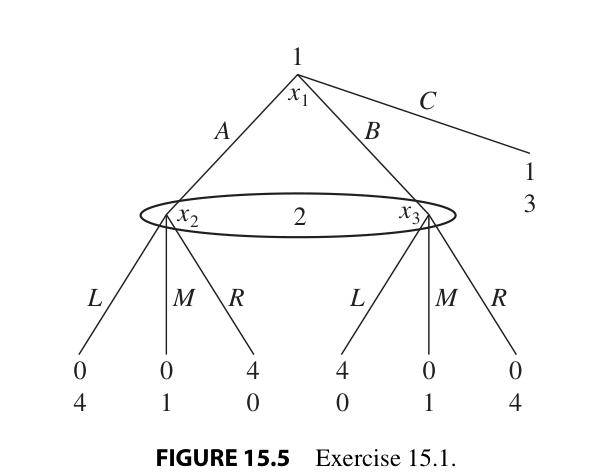
\includegraphics[keepaspectratio,alt={Figure 15.5 Exercise 15.1}]{../figures/tadelis-15-5.png}}



\textbf{FIGURE 15.5} Exercise 15.1.

\end{quote}

